% ==========================================
% BAB II STUDI LITERATUR
% ==========================================
\chapter{STUDI LITERATUR}
\label{chap:studi-literatur}
\section{Sistem Tiket Elektronik (\textit{E-Ticket})}
\subsection{Definisi dan Evolusi \textit{E-Ticket}}
... (Penjelasan mengenai pergeseran dari tiket konvensional ke digital, serta definisi formal dari \textit{e-ticket} berdasarkan literatur akan ditambahkan di sini) ...

\subsection{Peran QR Code dalam Sistem \textit{E-Ticket}}
... (Penjelasan mengenai mengapa QR Code menjadi teknologi yang dominan untuk implementasi \textit{e-ticket}, mencakup kemudahan penggunaan dan adopsi luas akan ditambahkan di sini) ...

\section{Teknologi \textit{Quick Response (QR) Code}}
\subsection{Sejarah dan Prinsip Kerja QR Code}
... (Penjelasan singkat mengenai sejarah penciptaan oleh Denso Wave dan cara kerja dasarnya dalam menyimpan data akan ditambahkan di sini) ...

\subsection{Struktur dan Jenis QR Code}
... (Pembahasan mengenai komponen teknis QR Code seperti zona tenang, pola pencari, dan kapasitas data. Juga akan dibedakan antara QR Code Statis dan Dinamis dalam konteks pemasaran untuk mengklarifikasi perbedaan dengan konsep TA ini) ...

\section{Keamanan Sistem \textit{E-Ticket}}
\subsection{Ancaman Keamanan pada \textit{E-Ticket} Berbasis QR Code Statis}
... (Identifikasi vektor-vektor serangan yang relevan dengan masalah, seperti pemalsuan, duplikasi, dan penyadapan akan ditambahkan di sini) ...

\subsection{Analisis Serangan Umum}
... (Pemberian definisi teknis dari serangan spesifik yang ingin diatasi, seperti \textit{Replay Attack} untuk masalah \textit{screenshot}, dan \textit{Forgery} untuk masalah pemalsuan tiket akan ditambahkan di sini) ...

\section{Landasan Teori Kriptografi untuk Solusi}
\subsection{Kriptografi Asimetris (\textit{Public-Key Cryptography})}
... (Penjelasan mengenai konsep dasar pasangan kunci publik dan privat sebagai fondasi untuk teknologi selanjutnya akan ditambahkan di sini) ...

\subsection{Tanda Tangan Digital (\textit{Digital Signature})}
... (Penjelasan mendetail mengenai cara kerja Tanda Tangan Digital untuk menjamin otentisitas, integritas, dan nirsangkal. Ini adalah pilar untuk aspek \textbf{Secure}) ...

\subsection{\textit{Time-based One-Time Password} (TOTP)}
... (Penjelasan mengenai mekanisme TOTP berdasarkan standar RFC 6238, yang menggunakan kunci rahasia bersama dan waktu sebagai faktor. Ini adalah pilar untuk aspek \textbf{Dynamic}) ...

\section{Penelitian Terkait (\textit{State-of-the-Art})}
\subsection{Tinjauan Sistem Keamanan \textit{E-Ticket} yang Sudah Ada}
... (Rangkuman penelitian atau implementasi lain yang mencoba mengamankan \textit{e-ticket}, beserta kelebihan dan kekurangannya akan ditambahkan di sini) ...

\subsection{Tinjauan Pemanfaatan Kriptografi pada QR Code}
... (Rangkuman penelitian lain yang telah menerapkan enkripsi atau Tanda Tangan Digital pada QR Code untuk berbagai kasus penggunaan akan ditambahkan di sini) ...

\subsection{Celah Penelitian (\textit{Research Gap}) dan Posisi Penelitian Ini}
... (Kesimpulan dari tinjauan sebelumnya yang menunjukkan apa yang belum ditangani oleh penelitian lain, dan menegaskan bahwa sintesis unik antara Tanda Tangan Digital dan TOTP untuk mengatasi ancaman ganda (pemalsuan dan duplikasi \textit{real-time}) pada \textit{e-ticket} adalah kontribusi utama dari Tugas Akhir ini) ...

\section{Penulisan Gambar, Tabel, Rumus, dan Kode}
\lipsum[1]

\subsection{Gambar}
Contoh gambar dapat dilihat pada Gambar \ref{gambar:jaringan}. Gambar dan judulnya diposisikan di tengah. Nomor gambar tidak diakhiri tanda titik. Gambar tersebut dibuat menggunakan aplikasi draw.io dan disimpan ke format PNG setelah dengan zoom setting pada angka 300\%. Ukuran gambar yang ditampilkan dapat diatur dengan mengubah nilai \textit{width} dalam sintaks \textit{includegraphics}.

\begin{figure}[t] % pilihan opsi yang disarankan: t = top, b = bottom, h = here
	\centering
  \captionsetup{justification=centering}
    	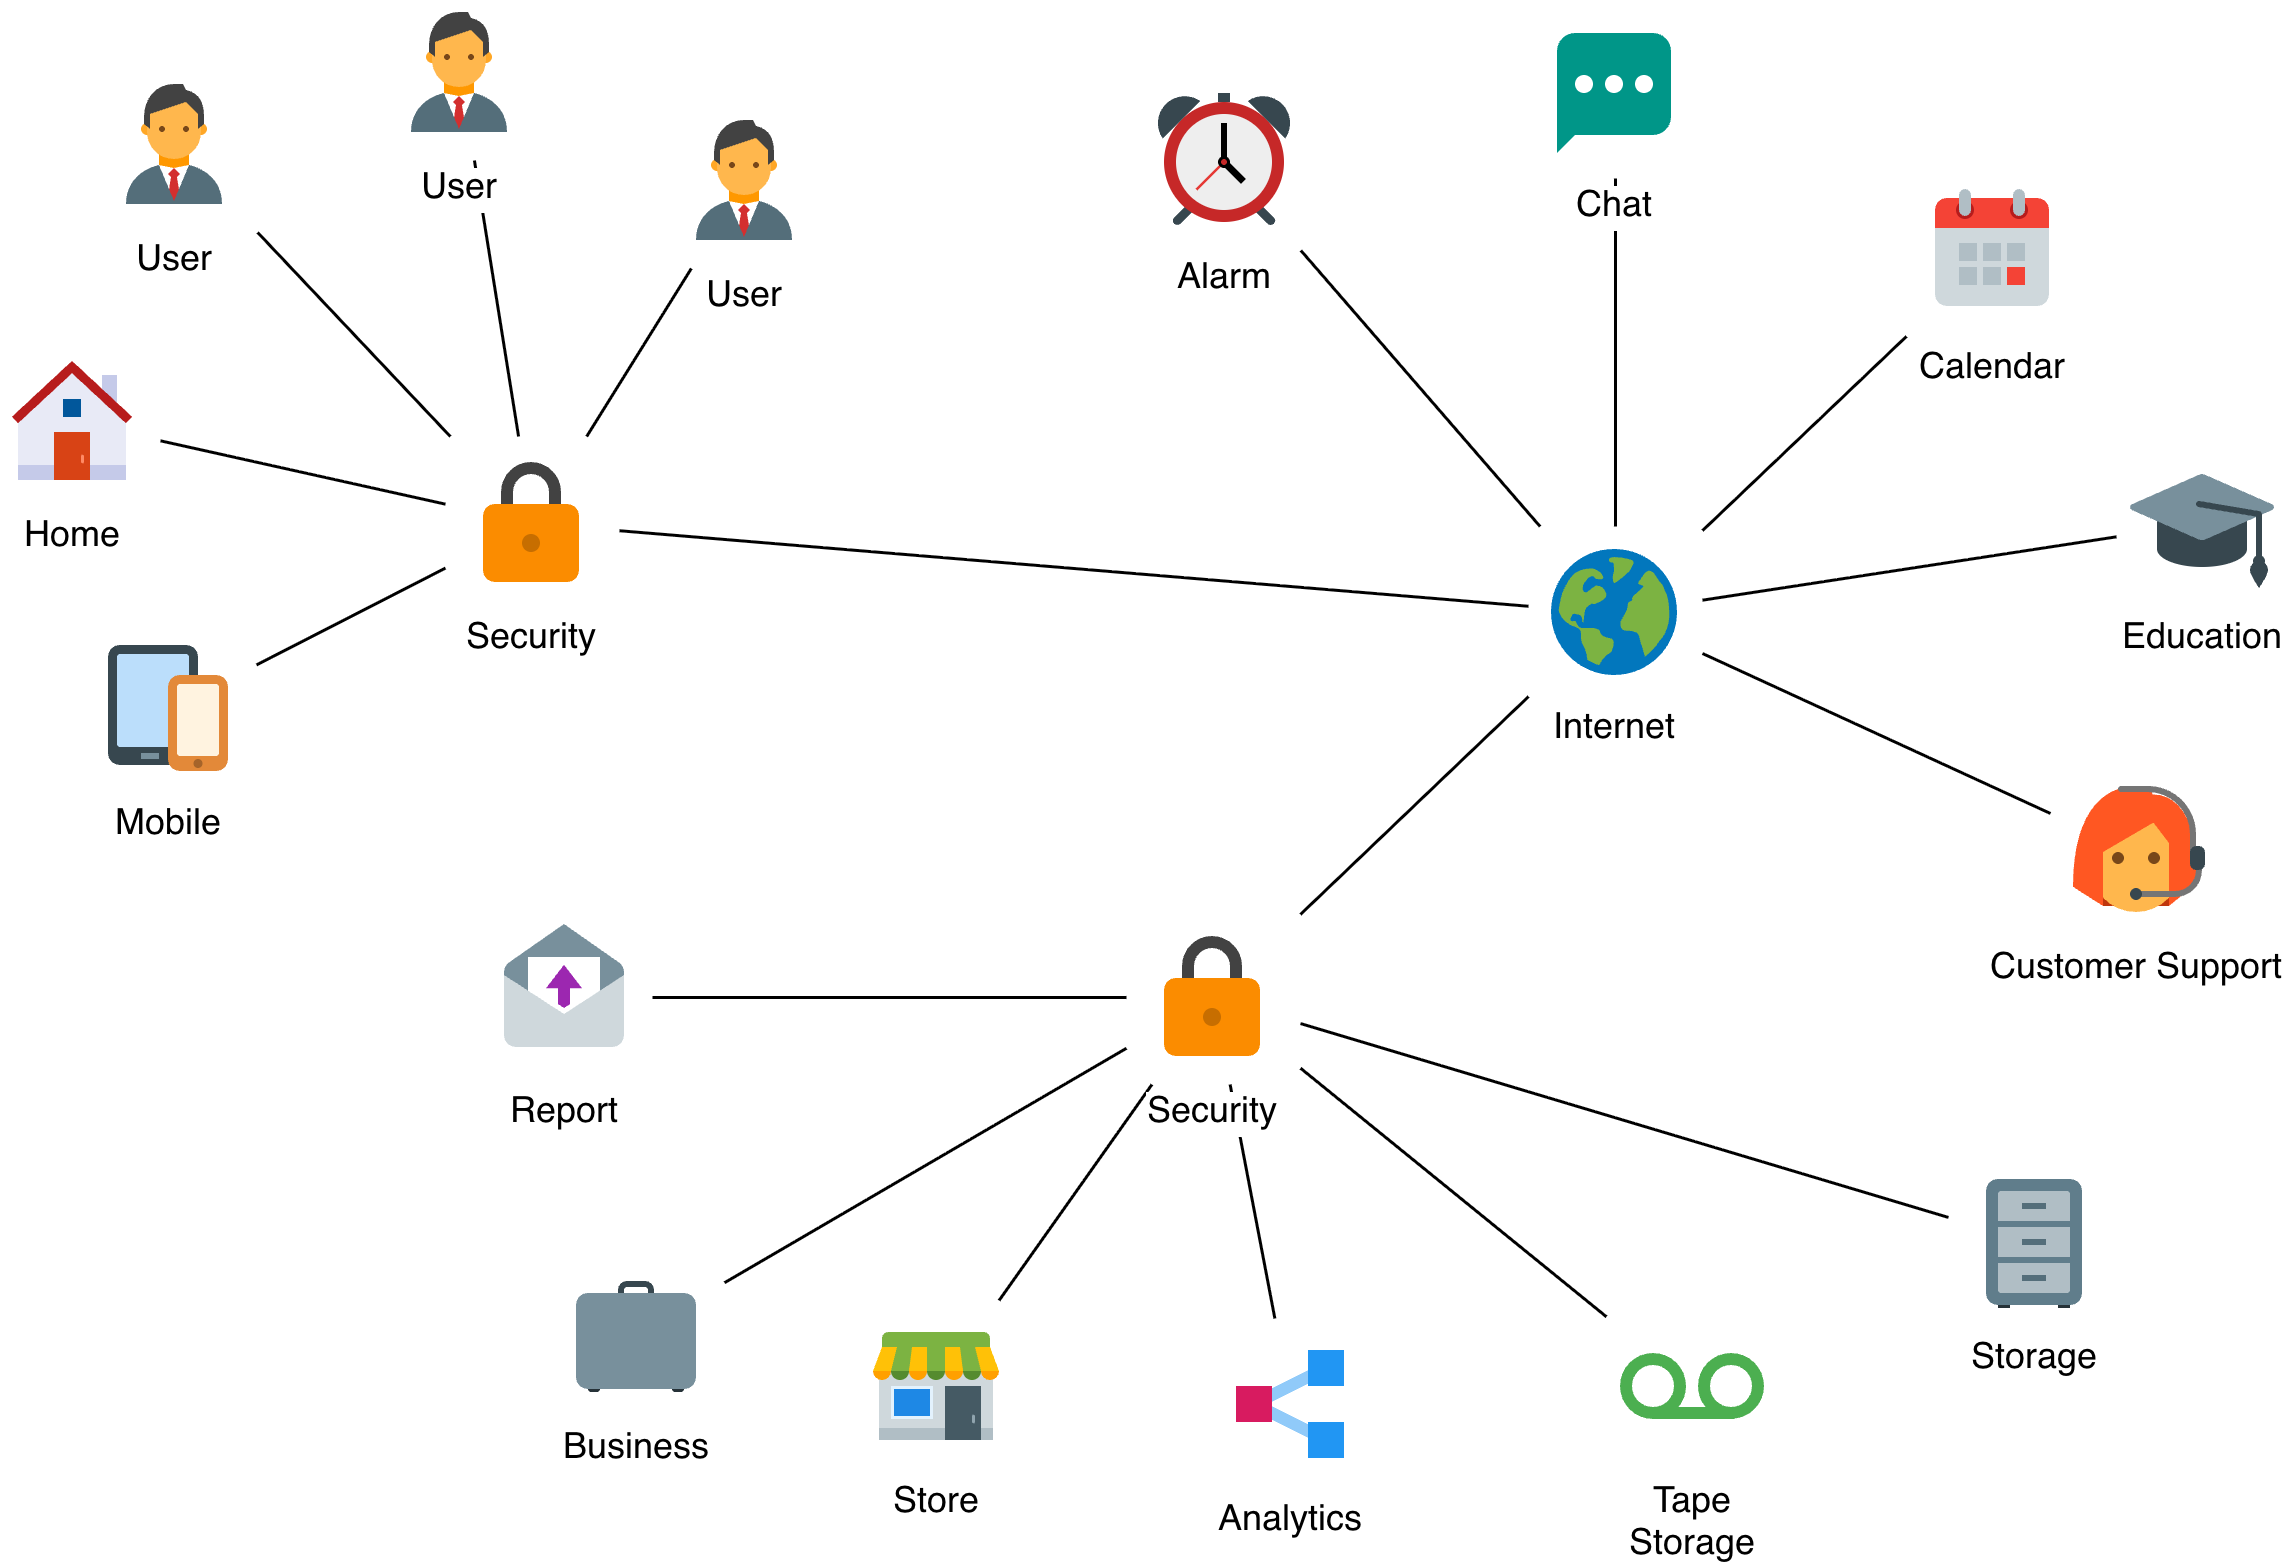
\includegraphics[width=0.7\textwidth]{image/gambar1.png}
	\caption{Contoh gambar jaringan}
	\label{gambar:jaringan}
\end{figure}

Gambar umumnya tidak jelas atau kabur jika gambar tersebut:
\begin{enumerate}[a.]
  \item diperoleh dari hasil cropping pada suatu halaman buku atau situs web;
  \item hasil pembesaran gambar yang gambar aslinya sebenarnya berukuran kecil; atau
  \item disimpan dalam resolusi kecil
\end{enumerate}
Ketidakjelasan gambar ini dapat dilihat pada garis-garis diagram yang tidak tegas dan tulisan-tulisan dalam gambar yang tampak kabur dan kurang jelas terbaca.

Untuk mendapatkan gambar yang tidak kabur (\textit{blur}), langkah-langkah berikut dapat digunakan:
\begin{enumerate}[(a)]
\item Gambar yang didapat di suatu pustaka atau referensi sebaiknya digambar ulang, misalnya menggunakan PowerPoint, Canva, Figma, draw.io, atau yang lainnya.
\item Jika diagram atau ilustrasi digambar menggunakan draw.io, saat gambar disimpan ke format PNG atau JPG (\textit{export as}), lakukan \textit{zoom} ke minimal 300\% (\textit{the default value is} 100\%). 
\item Jika diagram digambar dengan menggunakan PowerPoint, gambar dapat langsung di-\textit{copy-paste} ke Word.
\end{enumerate}

\subsection{Tabel}
Tabel ada dua jenis, yaitu tabel yang bisa termuat dalam satu halaman dan tabel yang sangat panjang sehingga tidak muat dalam satu halaman.
\subsubsection{Tabel yang Muat dalam Satu Halaman}
Contoh tabel dapat dilihat pada Tabel \ref{tbl:harga1} dan \ref{tbl:harga2}. Tabel dan judulnya dibuat rata kiri dan judul tabel diletakkan di atas tabel. Usahakan tabel dapat ditulis dalam satu halaman, tidak terpotong ke halaman berikutnya.

\begin{table}[t] % pilihan opsi yang disarankan: t = top, b = bottom, h = here
  \begin{tabular}{ | p{2cm} | p{2cm} | p{3cm} |}
	\hline
	Nama 	& Satuan 		& Harga \\
	\hline
	Buku 	& Exemplar	& 25000 \\
	Komputer	& Unit		& 2500000 \\
	Pensil	& Buah		& 118900 \\
	\hline
	\end{tabular}
\caption{Tabel harga bahan pokok}
\label{tbl:harga1}
\end{table}

\begin{table}[t] % pilihan opsi yang disarankan: t = top, b = bottom, h = here
	\begin{tabular}{ | l | c | r | }
	\hline
	Nama 	& Satuan 		& Harga \\
	\hline
	Buku 	& Exemplar	& 25000 \\
	Komputer	& Unit		& 2500000 \\
	Pensil	& Buah		& 118900 \\
	\hline
	\end{tabular}
\caption{Tabel harga bahan sekunder}
\label{tbl:harga2}
\end{table}

\subsubsection{Tabel yang Sangat Panjang}
Jika tabel terlalu panjang sehingga tidak muat dalam satu halaman, gunakan paket 
\textit{longtable} untuk membuat tabel yang dapat terpotong ke halaman berikutnya, 
seperti pada Tabel \ref{tbl:longtable1}.

\begin{longtable}{@{\extracolsep{\fill}} l c r r}
\caption{Comprehensive Data Table Example}\label{tbl:longtable1} \\
\toprule
\textbf{ID} & \textbf{Name} & \textbf{Score} & \textbf{Rank} \\
\midrule
\endfirsthead

\caption*{Comprehensive Data Table Example (lanjutan)} \\
\toprule
\textbf{ID} & \textbf{Name} & \textbf{Score} & \textbf{Rank} \\
\midrule
\endhead

\midrule
\multicolumn{4}{r}{\textit{Bersambung ke halaman berikutnya}} \\
\bottomrule
\endfoot

\bottomrule
\endlastfoot

% === Table Data ===
1 & Alice Smith & 89 & 5 \\
2 & Bob Johnson & 93 & 3 \\
3 & Carol Davis & 95 & 2 \\
4 & Daniel Wilson & 88 & 6 \\
5 & Eve Thompson & 97 & 1 \\
6 & Frank Brown & 85 & 7 \\
7 & Grace Lee & 91 & 4 \\
8 & Henry Miller & 80 & 9 \\
9 & Irene Garcia & 83 & 8 \\
10 & Jack Robinson & 78 & 10 \\
% Repeat with more rows to make it long
11 & Kevin Harris & 76 & 11 \\
12 & Laura Martin & 75 & 12 \\
13 & Michael Clark & 74 & 13 \\
14 & Natalie Lewis & 73 & 14 \\
15 & Olivia Walker & 72 & 15 \\
16 & Peter Hall & 71 & 16 \\
17 & Quinn Allen & 70 & 17 \\
18 & Rachel Young & 69 & 18 \\
19 & Samuel King & 68 & 19 \\
20 & Tina Wright & 67 & 20 \\
21 & Uma Scott & 66 & 21 \\
22 & Victor Green & 65 & 22 \\
23 & Wendy Adams & 64 & 23 \\
24 & Xavier Nelson & 63 & 24 \\
25 & Yolanda Carter & 62 & 25 \\
26 & Zachary Perez & 61 & 26 \\
27 & Amelia Baker & 60 & 27 \\
28 & Benjamin Rivera & 59 & 28 \\
29 & Charlotte Rogers & 58 & 29 \\
30 & David Murphy & 57 & 30 \\
31 & Ethan Cooper & 56 & 31 \\
32 & Fiona Reed & 55 & 32 \\
33 & George Bailey & 54 & 33 \\
34 & Hannah Cox & 53 & 34 \\
35 & Isaac Howard & 52 & 35 \\
36 & Julia Ward & 51 & 36 \\
37 & Kyle Flores & 50 & 37 \\
38 & Lily Bell & 49 & 38 \\
39 & Mason Sanders & 48 & 39 \\
40 & Nora Patterson & 47 & 40 \\
41 & Owen Ramirez & 46 & 41 \\
42 & Penelope Torres & 45 & 42 \\
43 & Quentin Foster & 44 & 43 \\
44 & Rebecca Gonzales & 43 & 44 \\
45 & Sebastian Bryant & 42 & 45 \\
46 & Taylor Alexander & 41 & 46 \\
47 & Ursula Russell & 40 & 47 \\
48 & Vincent Griffin & 39 & 48 \\
49 & William Diaz & 38 & 49 \\
50 & Zoe Simmons & 37 & 50 \\
% (You can easily extend this list to hundreds of rows)
\end{longtable}

\subsubsection{Rumus}
Contoh rumus matematika dapat ditulis seperti pada Persamaan \ref{eq:contoh1} di bawah ini. 
Penomoran persamaan diletakkan di sebelah kanan, dan rumus ditulis dalam mode \textit{display math}.
\begin{equation}
E = mc^2
\label{eq:contoh1}
\end{equation}

Contoh lain penulisan rumus matematika yang lebih kompleks dapat ditulis seperti pada Persamaan \ref{eq:rumus2}.

\begin{align}
f(x) &= ax^2 + bx + c \\
f'(x) &= \frac{d}{dx}(ax^2 + bx + c) \notag \\ % tidak menampilkan nomor pada baris ini
      &= 2ax + b \label{eq:rumus2}
\end{align}

Jika rumus terlalu panjang untuk ditulis dalam satu baris, gunakan lingkungan \textit{multline} seperti pada Persamaan \ref{eq:rumus3} di bawah ini.
\begin{multline} 
y = a_0 + a_1x + a_2x^2 + a_3x^3 + a_4x^4 + a_5x^5 + a_6x^6 + a_7x^7 \\
    + a_8x^8 + a_9x^9 + a_{10}x^{10} \label{eq:rumus3}
\end{multline}

Jika ada penurunan rumus yang terdiri dari beberapa baris, namun tidak memerlukan penomoran pada setiap baris, gunakan lingkungan \textit{align*}, misalnya:

\begin{align*} 
S &= \sum_{i=1}^{n} i^2 \\
  &= 1^2 + 2^2 + 3^2 + \cdots + n^2 \\
  &= \frac{n(n + 1)(2n + 1)}{6}
\intertext{Contoh lainnya adalah rumus untuk mencari nilai rata-rata fungsi $f(x)$ pada interval $[p, q]$:}
\bar{f} &= \frac{1}{q - p} \int_{p}^{q} f(x) \, dx \\
        &= \frac{1}{q - p} \int_{p}^{q} (ax^2 + bx + c) \, dx \\
        &= \frac{1}{q - p} \left[ \frac{a}{3}x^3 + \frac{b}{2}x^2 + cx \right]_p^q \\
        &= \frac{a(q^3 - p^3)}{3(q - p)} + \frac{b(q^2 - p^2)}{2(q - p)} + c \label{eq:rumus4}
\end{align*}



\subsection{Algoritma, Pseudocode, atau Kode}
Contoh penulisan algoritma atau pseudocode dapat ditulis seperti pada Kode \ref{alg:contoh1} di bawah ini. 
Gunakan paket \textit{listings} untuk menulis source code dalam bahasa pemrograman tertentu, seperti pada Kode \ref{lst:contoh1}. 


% -- Example of pseudocode and source code listing --
% -- Gunakan minipage agar listing tidak terpotong ke halaman berikutnya --
\begin{minipage}{\textwidth} 
\begin{lstlisting}[frame=lines, captionpos=t, caption={Contoh pseudocode}, label={alg:contoh1}]
ALGORITHM HelloWorld
   PRINT "Hello, World!"
END ALGORITHM
\end{lstlisting}
\end{minipage}

\begin{minipage}{\textwidth}
\begin{lstlisting}[language=Python, frame=single, caption={Contoh source code Python}, captionpos=t, label={lst:contoh1}]
def hello_world():
    print("Hello, World!")       
hello_world()
\end{lstlisting}
\end{minipage}


\section{Beberapa Kesalahan Penulisan yang Sering Terjadi}
\subsection{Penggunaan Kata "di mana" atau "dimana"}
Banyak yang menuliskan kata "di mana" atau "dimana" sebagai pengganti kata "which" dalam bahasa Inggris. 
Padahal, penggunaan kata "di mana" atau "dimana" tidak tepat dalam konteks tersebut. Demikian juga untuk kata serupa, misalnya "yang mana".
Kata "di mana" atau "dimana" ini harus diganti dengan kata lain, seperti "dengan", "tempat", "yang", dan sebagainya tergantung kalimatnya.
Penjelasan lengkap dapat dilihat pada \autocite{BPBI}.

\subsection{Penggunaan Kata "sedangkan" dan "sehingga"}

\begin{table}[t]
  \begin{tabular}{|c|l|l|}
  \hline
  Kata & Salah & Benar \\ \hline
  sedangkan & \begin{tabular}[c]{@{}c@{}}Sedangkan sistem lama masih\\ digunakan oleh banyak pengguna.\end{tabular} & \begin{tabular}[c]{@{}c@{}}Sistem lama masih digunakan\\ oleh banyak pengguna,\\ sedangkan sistem baru belum siap.\end{tabular} \\ \hline
  sehingga & \begin{tabular}[c]{@{}c@{}}Sehingga sistem lama masih\\ digunakan oleh banyak pengguna.\end{tabular} & \begin{tabular}[c]{@{}c@{}}Sistem lama masih digunakan\\ oleh banyak pengguna sehingga\\ sistem baru belum siap.\end{tabular} \\ \hline
  \end{tabular}
  \caption{Contoh penggunaan kata "sedangkan" dan "sehingga"}
  \label{tbl:sedangkan_sehingga}
\end{table}

Kata "sedangkan" dan "sehingga" adalah kata hubung atau konjungsi. 
Konjungsi adalah kata atau ungkapan yang menghubungkan satuan bahasa 
(kata, frasa, klausa, dan kalimat). 
Konjungsi dapat dibagi menjadi konjungsi intrakalimat dan antarkalimat.  
Kata "sedangkan" menghubungkan dua klausa yang bersifat kontrasif, 
sedangkan "sehingga" menghubungkan dua klausa yang bersifat kausal. 
Dalam ragam formal, kata hubung “sedangkan” dan “sehingga” hanya dapat digunakan 
sebagai konjungsi intrakalimat sehingga kedua konjungsi itu \textbf{tidak dapat diletakkan pada awal kalimat}.
Selain itu, penggunaan kata "sedangkan" harus didahului oleh koma (,), sedangkan kata "sehingga" tidak perlu didahului oleh koma (,).
Contoh penggunaan yang benar dan salah dapat dilihat pada Tabel \ref{tbl:sedangkan_sehingga}.


\subsection{Penggunaan Istilah yang Tidak Baku}
Ada beberapa istilah yang sering digunakan dalam pembicaraan sehari-hari, tetapi tidak baku dalam penulisan ilmiah.
Beberapa istilah tersebut antara lain:
\begin{enumerate}
  \item analisa $\rightarrow$ analisis
  \item eksisting atau existing $\rightarrow$ yang ada atau saat ini
  \item bisnis proses $\rightarrow$ proses bisnis
  \item user $\rightarrow$ pengguna
  \item system $\rightarrow$ sistem
  \item database $\rightarrow$ basis data
  \item aktifitas $\rightarrow$ aktivitas
  \item efektifitas $\rightarrow$ efektivitas
  \item sosial media $\rightarrow$ media sosial
\end{enumerate}

\subsection{Pemisah Desimal dan Ribuan}
Tanda pemisah desimal dalam bahasa Indonesia adalah tanda koma, contoh:
\begin{enumerate}
  \item (Salah) Akurasi naik menjadi 50.6\% 
  \item (Benar) Akurasi naik menjadi 50,6\% 
\end{enumerate}

\subsection{Daftar atau \textit{List}}
Ada beberapa aturan penulisan daftar atau \textit{list} yang perlu diperhatikan, antara lain:
\begin{enumerate}[a)]
\item Jika memungkinkan, hindari penggunaan “bullet points” atau sejenisnya. Sebaiknya, gunakan angka (1, 2, 3, ...) atau huruf (a, b, c, …). Dengan demikian, pembaca dapat dengan mudah melihat jumlah \textit{item} atau \textit{list}. 
\item Jika dalam daftar hanya ada satu item, tidak perlu menggunakan nomor urut.
\item Penjelasan atau deskripsi suatu item sebaiknya menyatu dengan judul item tersebut, tidak berbeda halaman. Contoh yang salah: judul item ada di halaman 10, namun deskripsinya di halaman 11. Sebaiknya pindahkan judul tersebut ke halaman 11.
\item Jika penjelasan atau deskripsi suatu item cukup panjang, misalnya lebih dari 1 halaman atau terdiri atas beberapa paragraf, sebaiknya setiap item tersebut dijadikan judul subbab, kecuali jika level subbab sudah mencapai level 4. 
\end{enumerate}

\subsection{Penggunaan Kata "masing-masing" dan "setiap"}
Kata “masing-masing” digunakan di belakang kata yang diterangkan, misalnya 
"Setiap proses menggunakan algoritma masing-masing". Kata “tiap-tiap” atau “setiap”
ditempatkan di depan kata yang diterangkan, misalnya
"Setiap proses menggunakan algoritma tertentu".
